% Template for ICASSP-2018 paper; to be used with:
%          spconf.sty  - ICASSP/ICIP LaTeX style file, and
%          IEEEbib.bst - IEEE bibliography style file.
% --------------------------------------------------------------------------
\documentclass{article}
  \usepackage{spconf,amsmath,graphicx,amssymb, balance}

  % Example definitions.
  % --------------------
  \def\x{{\mathbf x}}
  \def\L{{\cal L}}

  % Title.
  % ------
  \title{Quantifying Graphical Password Strength by Neural Networks}
  %
  % Single address.
  % ---------------
 \name{Yushuo Guan, Yuanxing Zhang, Lin Chen$^*$, Kaigui Bian}
 \address{Peking University, $^*$Yale University}
  %
  % For example:
  % ------------
  %\address{School\\
  %	Department\\
  %	Address}
  %
  % Two addresses (uncomment and modify for two-address case).
  % ----------------------------------------------------------
%  \twoauthors
%   {Yushuo Guan, Yuanxing Zhang, Lin Chen$^*$, Kaigui Bian}
%{    Peking University, $^*$Yale University    }
%    { }
%    {
%    }
%  %
  \newtheorem{definition}{Definition}
  \begin{document}
  %\ninept
  %
  \maketitle
  %
  \begin{abstract}
  Graphical passwords have been widely used for protecting user privacy in many applications. Combining images and sketches in the design of graphical passwords could greatly increases the complexity for a regular user or a savvy shoulder-surfing attacker (that can record user inputs by video camera) to crack the password system. However, the recent advance in machine learning theory, e.g., the neural networks (NN), enables an attacker to make a better guess on the password by learning from user inputs, without the complete knowledge of the password system design. In this paper, we propose an NN-based framework of quantifying the graphical password strength against the shoulder-surfing attack. We present an NN-enabled attack model, and conduct experiments on four representative graphical password systems. Experimental results show that PIN and text passwords have serious security risks in presence of the shoulder-surfing attack, since the attack model can get a more than $90\%$ precision with less than $10$ training data.
  \end{abstract}
  %
  \begin{keywords}
  Graphical password, shoulder-surfing attack, neural network
  \end{keywords}
  %
  \section{Introduction}
  \label{sec:intro}

People are increasingly using graphical passwords to login their online accounts and access personal information (e.g., to visit social networks like Facebook or Twitter). Graphical passwords are knowledge-based passwords, motivated by the idea that correlates images or sketches with the shared secret~\cite{DBLP:journals/csur/BiddleCO12}. The simplest implementation of graphical passwords is the Personal Identification Number (PIN) and text passwords, which directly uses numbers and characters to create a password. More advanced passwords add more types of symbols in the password design, like human faces or photos~\cite{Passfaces,DBLP:conf/uss/JermynMMRR99,DBLP:conf/soups/WiedenbeckWBBM05}.

The use of images and sketches in the password design improves the theoretical complexity for a regular user or a savvy shoulder-surfing attacker (that can record user inputs by video camera) to crack the password system. The shoulder-surfing attack, a.k.a. peeping attack, allows adversaries to observe all actions of humans on input terminals and interactions between humans (provers) and computers (verifiers)~\cite{DBLP:journals/iacr/LiS05,DBLP:journals/cacm/Anderson94a}. Attackers may utilize direct observation or high-resolution cameras to record passwords. The theoretical complexity of guessing the password will decrease quickly after a number of successive observations by the shoulder surfing attacker. For example, the theoretical complexity of guessing a text password will decrease to $O(1)$, if the attacker successfully observe the user input for only one-time.

The vulnerability of text password is that the user input is exactly equal to the password itself. That is why the password could be exposed when the shoulder-surfing attacker captures the user input for one time.
Hence, to defeat the shoulder surfing attack, many advanced graphical password systems seek to create a mapping function between the password and the user input---the user input is no longer equal to the password. The user has to do the mapping by translating the password in his/her mind to an user input on the keypad. As a result, it is largely insufficient for attackers to crack the password merely with the records of user inputs.


However, the advance in neural network (NN) allows the attacker with shoulder-surfing methods to make a better guess on the graphical password by learning the possible mapping functions between the user input on the keypad and the the password in the user's mind. The advantage of the NN model is that it does not require hand-crafted features but it can directly learn from the raw observations. More importantly, NN makes it possible to quantify the strength of passwords against shoulder-surfing attacks. Conventional qualitative analysis on password strength sends certain questionnaires to and collect feedbacks from a group of participants, which is coarse-grained and bias-prone. 

Recent work has focused on the invention of shoulder-surfing resistant authentication systems. Zhang et al. \cite{DBLPHK17} and Maiti et al. \cite{DBLPJW17} made shoulder-surfing resistant schemes for augmented reality; Luo and Yang \cite{DBLP:journals/mta/LuoY16} and Higashiyama et al. \cite{DBLPOF15} present authentication schemes for smartphones to prevent shoulder-surfing attacks. All these systems are evaluated by a small number of volunteers, which is less convincing than a quantitative analysis. In contrast, NN evaluates the robustness of the graphical password by the theoretical complexity without requiring the knowledge of the password design. Hitaj et al. \cite{DBLP:journals/corr/abs-1709-00440} and Melicher et al. \cite{DBLP:conf/uss/MelicherUSKBCC16} use generative adversarial networks \cite{DBLP:journals/corr/GoodfellowPMXWOCB14} and recurrent neural networks to crack passwords, but they only focus on guessing attacks and their models merely apply to text password systems.

In this paper, we propose a NN-based framework for analyzing the password strength against shoulder-surfing attack. We redefine a graphical password system in the new framework, and propose an indicator to measure password strength against the shoulder surfing attack. We then establish different NN models for graphical passwords with single or multiple bits of input. We verify the rationality of the proposed indicator of password strength and study the impact of NN's information expressivity on the indicator. We have released source code and relative datasets on GitHub\footnote{https://github.com/PkuDavidGuan/graphical-password}.


\section{System Model}\label{sec:preliminaries}

In this section, we first present basic definitions with respect to an authentication, and then introduce the architecture in the graphical password systems.

\subsection{Basic Definitions}
The two fundamental components in the authentication system are authentication challenge and answer \cite{DBLP:journals/corr/BlockiBD14}. To
login, users have to enter an answer into the system (like ``123456'') based on a given challenge (like ``Please
enter your password.").
\begin{definition}
\textbf{Authentication challenge $\vec c$ and challenge space $\mathbb{C}$}. $\vec c = [x_1, x_2,...,x_M]$ contains $M$-bit messages for computers (verifiers) to distinguish users from malicious impersonators. Challenge space contains all possible authentication challenges that one graphical password system can provide.
$|\mathbb{C}| = \prod\limits_{i=1}^{M}|S_x^i|$,
where $S_x^i$ contains all possible options for the $i$-th bit message of an authentication challenge.
\end{definition}

\begin{definition}
\textbf{Authentication answer $\vec a$ and answer space $\mathbb{A}$}. For an $N$-bit graphical password system, $\vec a = [y_1, y_2,...,y_N]$,
where $y_i$ is the $i$-th input of users in the authentication process. ($i \in [1, N], i \in \mathbb{N}$)
The answer space contains all possible authentication answers a certain user can provide:
$|\mathbb{A}| = \prod\limits_{i=1}^{N}|S_y^i|$,
where $S_y^i$ contains all possible options for the $i$-th input of an answer. The answer space for different users may be different.
\end{definition}

Given the definitions of authentication challenge and authentication answer, we can propose the definition of the authentication password.
\begin{definition}
\textbf{Authentication password $p$ and password space $\mathbb{P}$}. The passwords can be viewed as a mapping from challenge space to answer space:
$p:\mathbb{C}\rightarrow\mathbb{A}$. For a specific authentication challenge $\vec c \in \mathbb{C}$, $p(\vec c)$
    is the correct authentication answer. Password space contains all possible authentication passwords.
    $|\mathbb{P}|
    = |\mathbb{A}|^{|\mathbb{C}|}$.
\end{definition}

\subsection{Architecture of the graphical password system}
  \begin{figure}[htb]
    \centering
    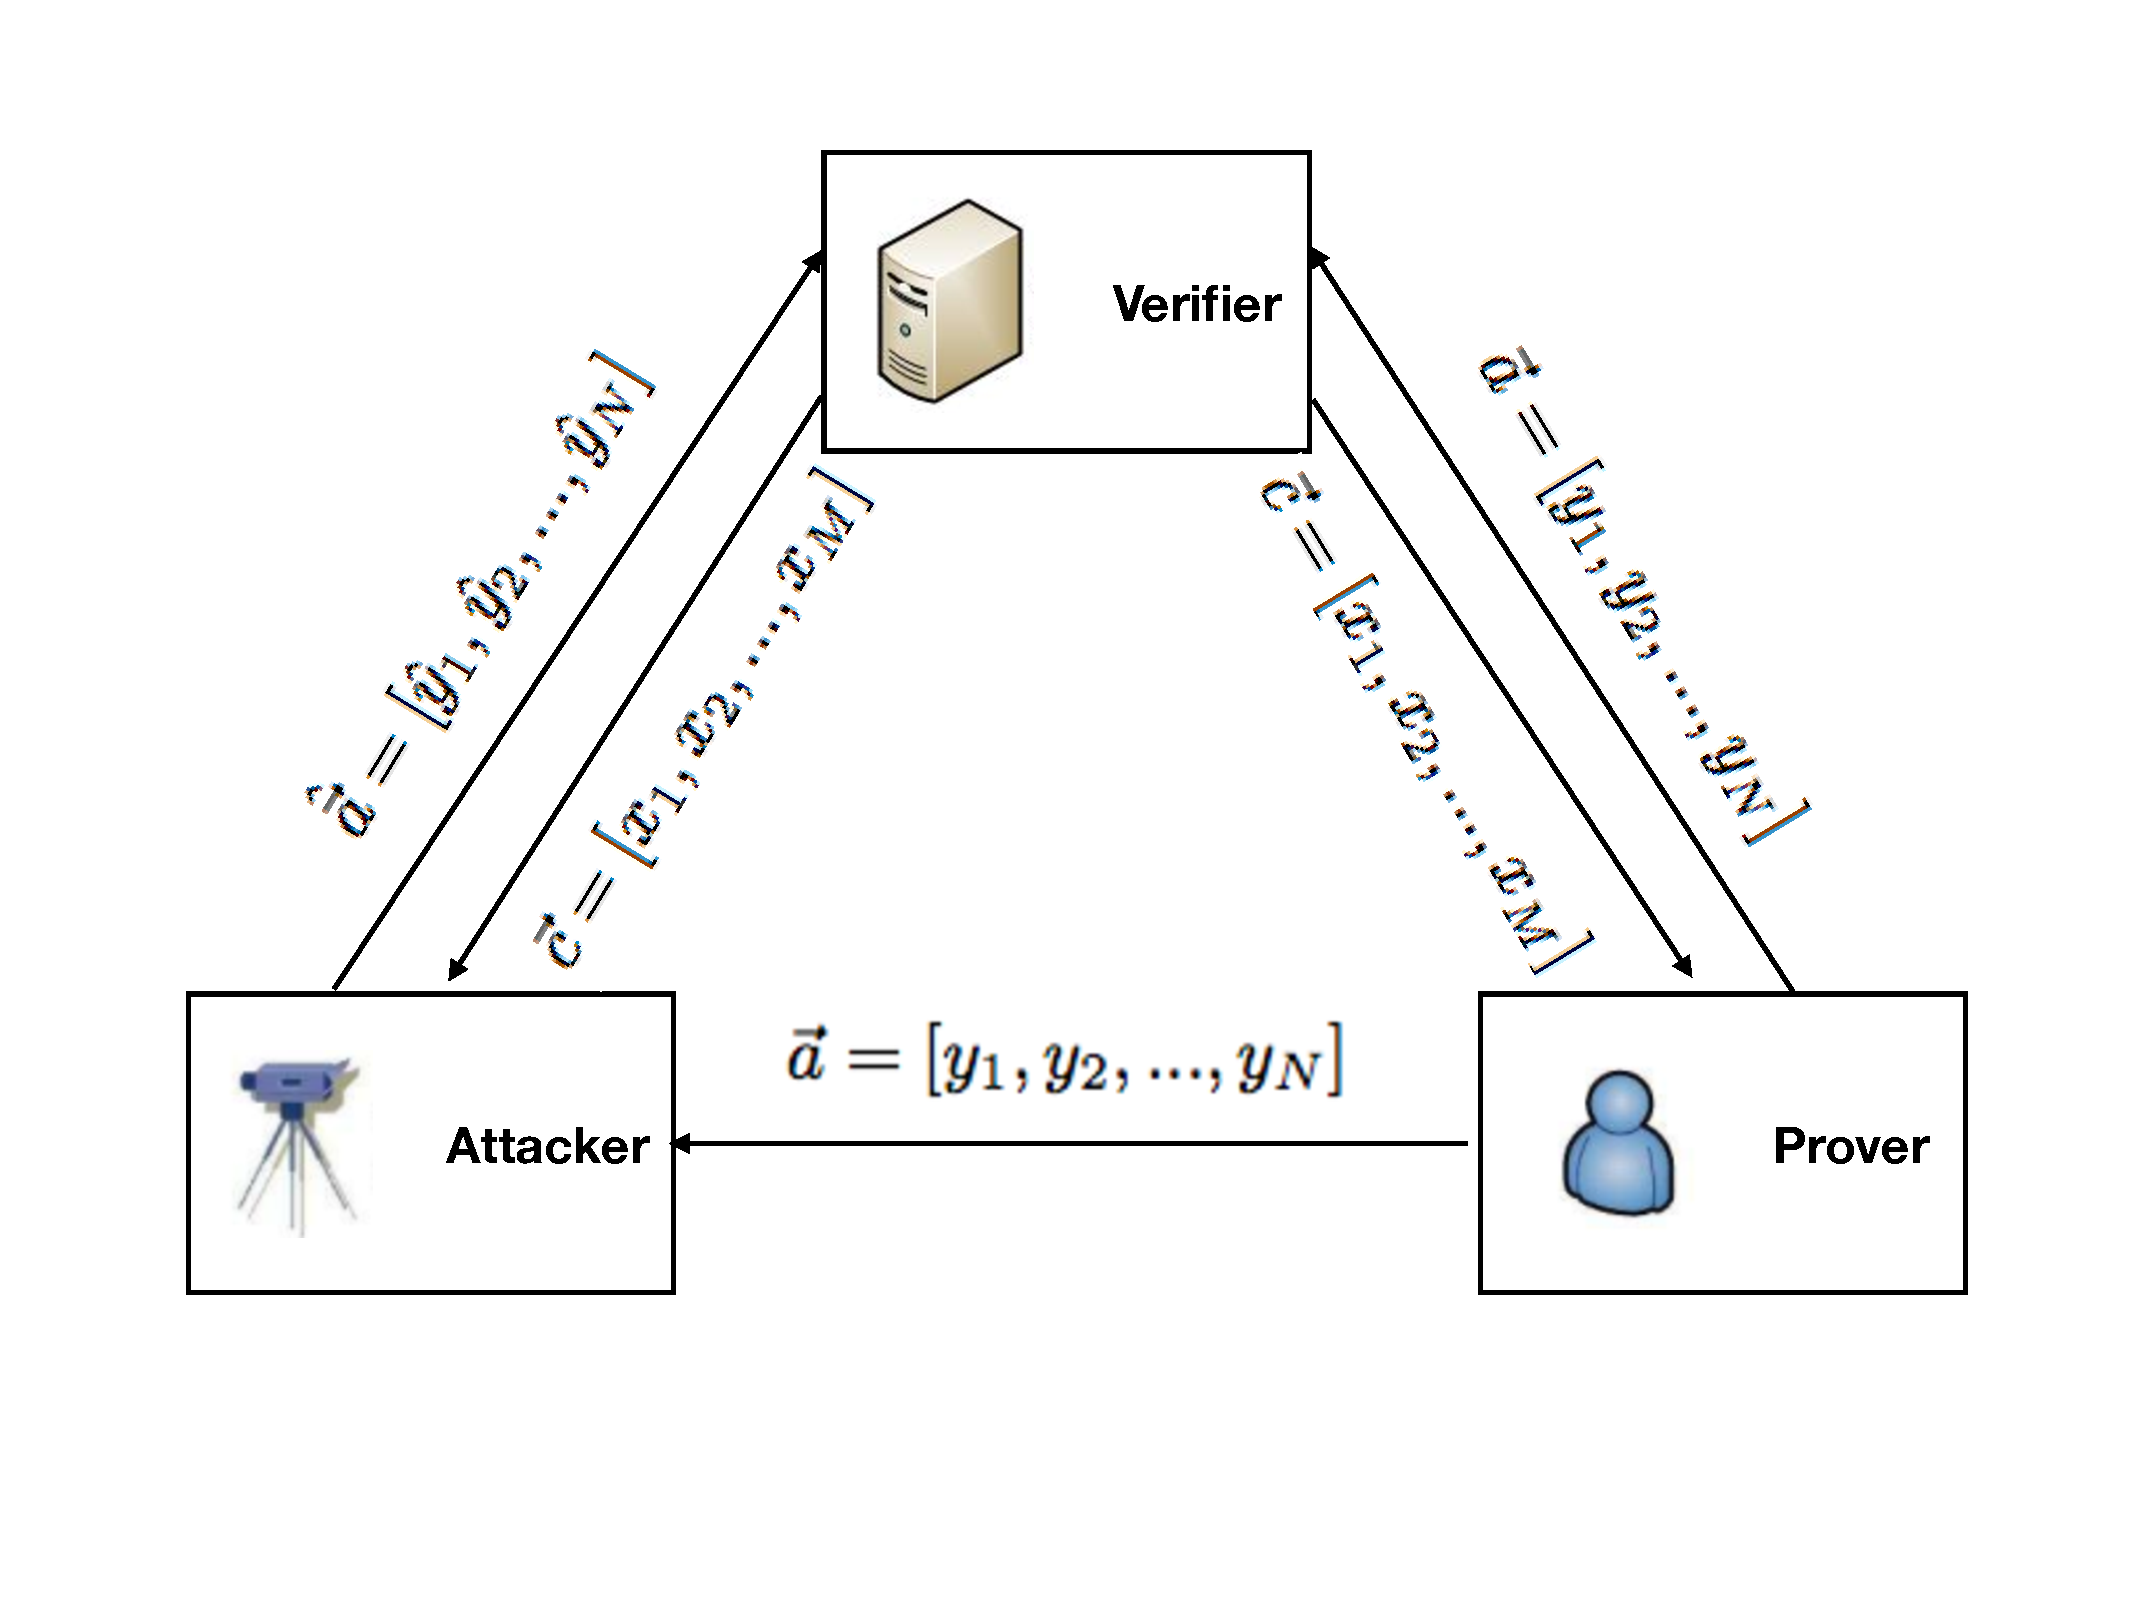
\includegraphics[width=8.5cm]{architecture.pdf}
    \caption{The architecture of a graphical password systems. }
    \label{fig:architecture} % XXX increase font size, logo png, http://www.iconpng.com
  \end{figure}

As shown in Figure~\ref{fig:architecture}, a graphical password system is composed of a verifier (computer), $K$ provers (human users), and an attacker.

The verifier is responsible for the verification of provers. It maintains $[p_1, p_2,...,p_{K}]$, which $p_i$ is the authentication password of prover $i$. In the authentication process, it generates $K$
authentication challenges $[\vec{c}_1, \vec{c}_2,...,\vec{c}_{K}]$ for each prover, and collects replies
$[\vec{a}_1,\vec{a}_2,...,\vec{a}_{K}]$ from each prover. The verifier distinguishes true provers $\mathbb{T}$
from attackers, where $\mathbb{T} = \{i|p_i(\vec{c}_i) = \vec{a}_i\}$.

For prover $i$, it gets an authentication challenge $\vec{c}_i$ from the verifier and replies with an authentication answer $\vec{a}_i = p_i(\vec{c}_i)$. Prover $i$ can login only if $i \in \mathbb{T}$.

The attacker hides himself in the system, records successive challenge-answer pairs $(\vec{c}, \vec{a})$, and trains the NN-based attack models against different provers. The result of an attack is determined by Equation~(\ref{equa:attacker}), and $\mathcal{A}(\vec{c}_i,\vec{a}_i)=1$ will be viewed as a successful attack on prover $i$.
\begin{equation}
    \mathcal{A}(\vec{c}, \vec{a})=
  \left\{
   \begin{aligned}
   1, \quad NN(\vec{c}) = \vec{a} \\
   0, \quad NN(\vec{c}) \neq \vec{a}
   \end{aligned}
   \right.
  \label{equa:attacker}
\end{equation}


\section{Design of the NN-based Attack Model}\label{sec:design}
In this section, we describe the design of an NN-based attack model.

% We start explaining the training methodology, and then present the hierarchy of the NN model used by the attacker model and enabled it to support different graphical password systems.

\subsection{The training procedure}
The first step for the attack model is to generate a training phase. Ideally, training data could be collected by the shoulder-surfing attackers. However, this approach is tim-consuming, as the training algorithm needs to wait until an attack is complete. To accelerate the process, we train the attack model by simulations that faithfully emulate the authentication process. The simulator maintains a verifier and a prover, which could generate authentication challenges and relevant answers successively.

\subsection{The NN-based attack model}
The input of the model is an $M$-dimensional vector  $\vec c = [x_1, x_2,...,x_M]$, which an authentication challenge. The output is simply a predicted $N$-bit answer with respect to the authentication challenge.

The input layer is simply $M$ units, i.e. one for each bit of an authentication challenge. The hierarchy of hidden layers is optional for attackers. The output layer differs between password designs.
\begin{itemize} 
  \item For the prediction of the $i$-bit authentication answer, if $S_y^i$ is known by attackers in advance, we will use a $|S_y^i|$-way softmax as predict the $i$-bit
  of the authentication answer.
  \item Otherwise, the softmax layer will be replaced by a regression layer. 
\end{itemize}
  The $i$-bit
  authentication answer can be predicted as:
  \begin{equation}
    \begin{gathered}
    a_i = (1-\mathcal{K}(S_y^i))(\sum_{i=1}^H w_ix_i) \\
    +\mathcal{K} (S_y^i)(\mathop{\arg\max}_{k \in S_y^i}\frac{exp(x_k)}{\sum_{j=1}^{S_y^i}exp(x_j)})
    \end{gathered}
  \end{equation}
  where $H$ is the size of the last hidden layer, $x_i$ is the output of the $i$-th unit in the last hidden layer.
  $\mathcal{K}(S_y^i) = 1$ when $S_y^i$ is known in advance, otherwise $\mathcal{K}(S_y^i) = 0$.




The NN-based attack model only focuses on the high precision, which means attackers could pass the authentication with a higher probability. The characteristics of the NN-based attack model distinguish itself from the conventional NN model, as the latter pay equal attention to precision and recall rates.

\subsection{Password strength indicator}
With the NN enabled attack model, we could quantify passwords strength against shoulder-surfing attacks from attackers' view, since the difficulty of NN training indirectly reflects password strength. Given the training set $R_{train}$ and test set $R_{test}$, we define an indicator to quantify the strength of password system $pass$ against the shoulder-surfing attack:
  \begin{equation}
    \begin{gathered}
    \mathcal{S}_{pass|l} = \mathop{\min}\ \ |R_{train}| \\
    s.t.\
    \forall (c,a) \in R_{test}, P(\mathcal{A}(c,a)=1|R_{train}) \geq l
    \end{gathered}
  \label{equa:indictor}
  \end{equation}

The indicator $\mathcal{S}_{pass|l}$ is highly influenced by the information expressivity of NN models. Therefore, for the rationality of the comparisons of password strength, the information expressivities of all NN models should be similar when $\mathcal{S}_{pass|l}$ is used to quantify multiple password systems at the same time.


\section{Evaluation}\label{sec:evaluation}
In this section, we first introduce two categories of advanced graphical password systems, and present our dataset and model architectures. We then conduct two experiments and study the rationality of the indicator $\mathcal{S}_{pass|l}$, and the impact of NN models' expressivity. The code of the experiment is available on Github (see \cite{gys} for details).

\subsection{Experiment setup}

\textbf{Advanced graphical password systems:} Advanced graphical passwords can be divided into two main categories based on recall and recognition \cite{Raaijmakers1992Models}.

Recognition-based systems generally ask users to memorize a portfolio of images during password creation and then recognize their images from among decoys \cite{DBLP:journals/csur/BiddleCO12,DBLP:journals/ijics/Renaud09}. PassFaces~\cite{Passfaces} is the canonical example of recognition-based graphical passwords. PassFaces has a pool of $F$ human face pictures, where users pre-select $A$ human faces. During login, a panel of $B$ candidate faces is presented. Users must select the face belonging to their set from among decoys. A number of $C$ such rounds are repeated with different panels (generally $C < A$).

Recall-based graphical password systems are referred to as drawmetric systems \cite{DBLP:journals/ijmms/AngeliCJR05}. In the recall-based systems, users recall the pattern they selected before and calculate an authentication answer based on the pattern. GrIDsure~\cite{Brostoff2010Evaluating} is a kind of recall-based graphical password system, which displays digits in a $D \times D$ grid. Users select and memorize a pattern consisting of an ordered subset of $E$ grid squares in advance. On subsequent logins, digits are randomly displayed within the grid squares, and users enter the sum of digits within their memorized pattern.

\textbf{Setup:}
We conduct experiments on $6$-bit PIN, indefinite length ($\leq 12$) text password, PassFaces, and GrIDsure. 
Note that the $6$-bit PIN has been widely used in ATM and online payment environments, and indefinite length text passwords are applied in social applications, like Facebook and Twitter. These are two representative types of conventional graphical password systems. %Passfaces and GrIDsure are two canonical examples of advanced graphical passwords. 
In the experiments, we set the following parameters $A = 5, B = 9, C = 1, D = 3, E = 4, F=100$.

\textbf{Attack model:}
We use Keras~\cite{chollet2015keras} to construct attack models for these four graphical passwords. There are two hidden layers for all attack models, and each layer has an identical number of hidden units. Identical hidden layers ensure that the four NN models have similar information expressivity. The number of units in the input and output layers is determined by the size of authentication challenges, and answers of different password systems, which makes little influence on the information expressivity. In the training process, we train each NN model with 10 different training sets, and compute the average precision. We use RMSProp as the optimizer.

\subsection{Experimental results}
\textbf{Rationality:}
In the first experiment, we seek to verify the rationality of our indicator $\mathcal{S}_{pass|l}$. All the NN models in this experiment have two hidden layers, and each layer has $32$ hidden units. We record the precision rate of four attack models, given different sizes of training sets.
  \begin{figure}[htb]
    \centering
    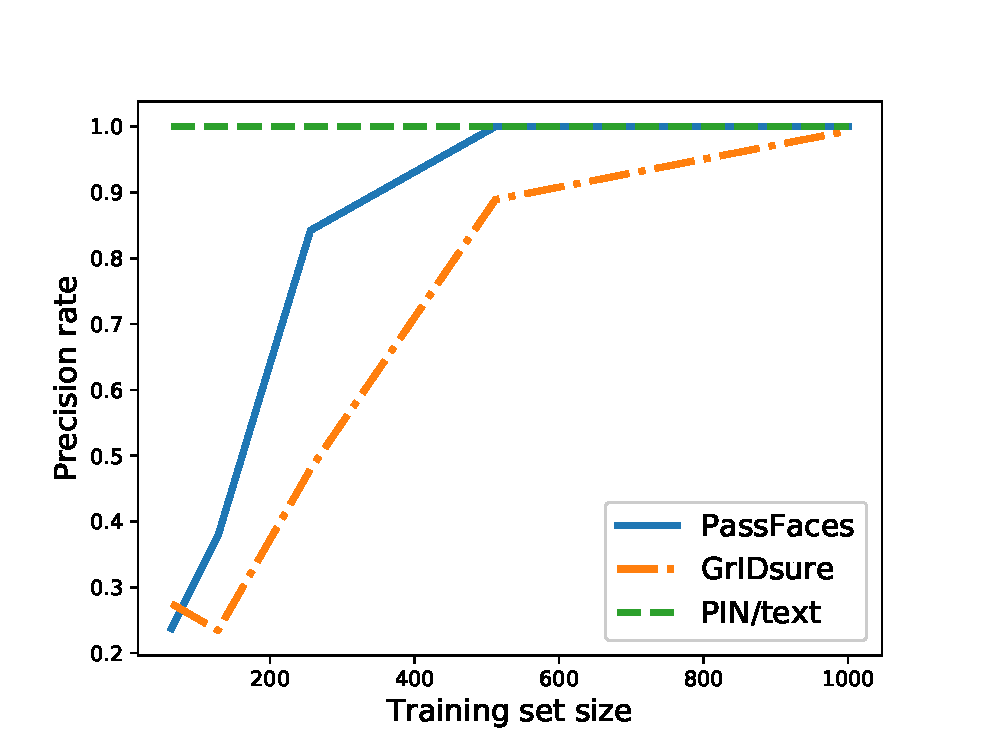
\includegraphics[width=8.5cm]{line}
    \caption{The precision of different graphical passwords, given different sizes of the training set. %XXX remove 0.9 line.
    } 
    \label{fig:results}
  \end{figure}

The result is shown in Figure~\ref{fig:results}. To achieve a $90\%$ precision or higher, the NN models for PIN/text need really small training set, the NN model for PassFaces need $256$ pieces of training data, and about $500$ pieces of training data are needed for GrIDsure. The result shows that GrIDsure and PassFaces have a better robustness than PIN/text passwords against the shoulder-surfing attack, and GrIDsure is even better than PassFaces.

The experimental result is consistent with the analytical result. The challenge space $\mathbb{C}$, and the answer space $\mathbb{A}$ of PIN and text passwords are zero-dimension. So, the authentication passwords in these systems are constant functions, which are vulnerable to the shoulder-surfing attack. For PassFaces,
$|\mathbb{C}| = \binom{F}{B}, |\mathbb{A}| = \binom{A}{C}$,
and the authentication password is an injective function, which is more difficult for NN-based models to crack. GrIDsure has an even larger challenge space and answer space, so it is less vulnerable to the attack.

  The result also reveals the high vulnerability of PIN and text passwords in the presence of the shoulder-surfing attack. Although these two traditional password systems are widely adopted in mobile devices, which may lead to severe security risks.

% This is what we think the Internet industry really has to pay attention.

\textbf{Comparisons of multiple NN models:}
In the second experiment, we build up several NN models with different information expressivities, and study their influence on the indicator $\mathcal{S}_{pass|l}$.
  \begin{figure}[htb]
    \centering
    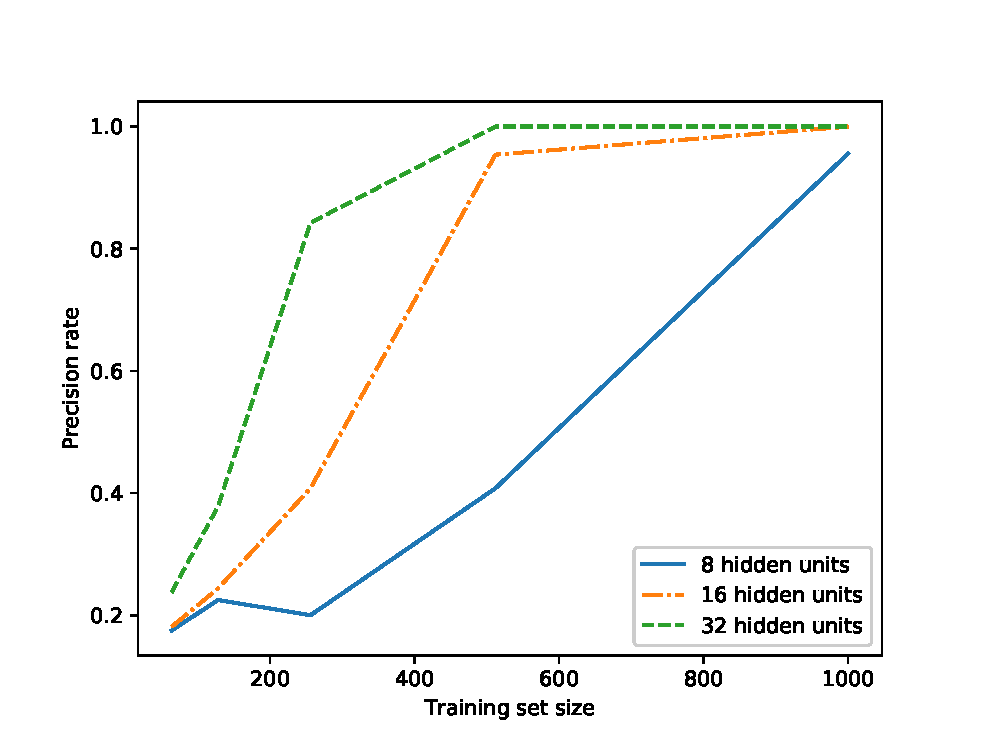
\includegraphics[width=8.5cm]{passfaces}
    \caption{The impact of information expressivity on PassFaces's NN model. }
    \label{fig:results2}
  \end{figure}


Figure~\ref{fig:results2} shows the results on PassFaces and GrIDsure. When there is $8$ hidden units in each hidden layer, $\mathcal{S}_{PassFaces|0.9}$ approaches $1000$. However, $\mathcal{S}_{PassFaces|0.9}$ halves when the number of hidden units increases to $32$. The result on GrIDsure is similar, which is omitted here. The attack model cannot get a $90\%$ accuracy, even with $1000$ pieces of training data when there are $8$ hidden units each layer.

The second experiment shows that information expressivities of NN models can seriously affect the password strength $\mathcal{S}_{pass|l}$.
The result is interesting both for the attacker and the stakeholder: the shoulder-surfing attacker will be more efficient when using state-of-the-art NN models; meanwhile, for researchers, the architecture of the NN attack model can be borrowed when quantifying a password system.

%Otherwise the indicator will be meaningless.

\section{Conclusion} \label{sec:conclusion}
In this paper, we propose a neural network based framework for analyzing the graphical password strength against the shoulder-surfing attack. We cast the basic definitions of password systems into the framework, and present a NN-enabled attack model. We then conduct experiments on four representative graphical password systems; and study the rationality of the proposed indicator, as well as the impact of NN's information expressivity. Experimental results show that a more than $90\%$ precision can be achieved for the attack model to crack PIN/text passwords, with less than $10$ pieces of training data.  The results indicates that PIN and text passwords have serious security risks in presence of the shoulder-surfing attack. 


  % Below is an example of how to insert images. Delete the ``\vspace'' line,
  % uncomment the preceding line ``\centerline...'' and replace ``imageX.ps''
  % with a suitable PostScript file name.
  % -------------------------------------------------------------------------
  % \begin{figure}[htb]

  % \begin{minipage}[b]{1.0\linewidth}
  %   \centering
  %   \centerline{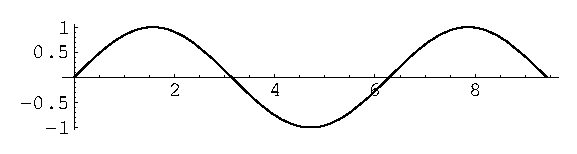
\includegraphics[width=8.5cm]{image1}}
  % %  \vspace{2.0cm}
  %   \centerline{(a) Result 1}\medskip
  % \end{minipage}
  % %
  % \begin{minipage}[b]{.48\linewidth}
  %   \centering
  %   \centerline{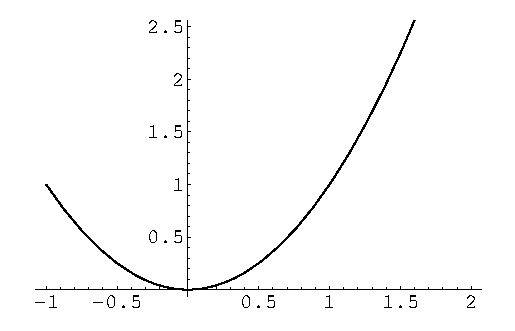
\includegraphics[width=4.0cm]{image3}}
  % %  \vspace{1.5cm}
  %   \centerline{(b) Results 3}\medskip
  % \end{minipage}
  % \hfill
  % \begin{minipage}[b]{0.48\linewidth}
  %   \centering
  %   \centerline{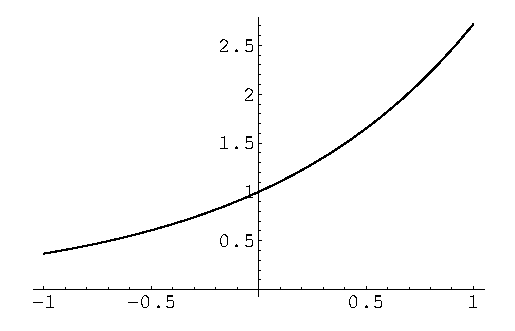
\includegraphics[width=4.0cm]{image4}}
  % %  \vspace{1.5cm}
  %   \centerline{(c) Result 4}\medskip
  % \end{minipage}
  % %
  % \caption{Example of placing a figure with experimental results.}
  % \label{fig:res}
  % %
  % \end{figure}


  % To start a new column (but not a new page) and help balance the last-page
  % column length use \vfill\pagebreak.
  % -------------------------------------------------------------------------
  %\vfill
  %\pagebreak


  \vfill\pagebreak


  % References should be produced using the bibtex program from suitable
  % BiBTeX files (here: strings, refs, manuals). The IEEEbib.bst bibliography
  % style file from IEEE produces unsorted bibliography list.
  % -------------------------------------------------------------------------
  \balance
  \bibliographystyle{IEEEbib}
  \bibliography{refs}

  \end{document}
